\section{Appendix}
\label{sec:appendix}



\begin{figure}[h]
    \centering
    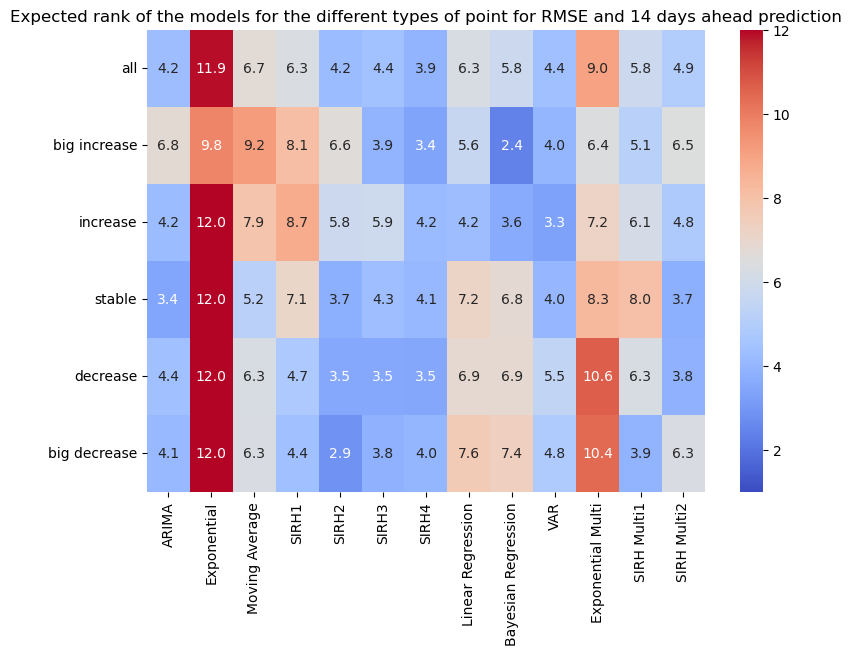
\includegraphics[width=0.7\textwidth]{figures/heatmap_RMSE_14.png}
    \caption{Expected rank of the models for each type of point for 14-days ahead predictions and RMSE loss}
    \label{fig:heatmap_RMSE_14}
\end{figure}

\begin{figure}[h]
    \centering
    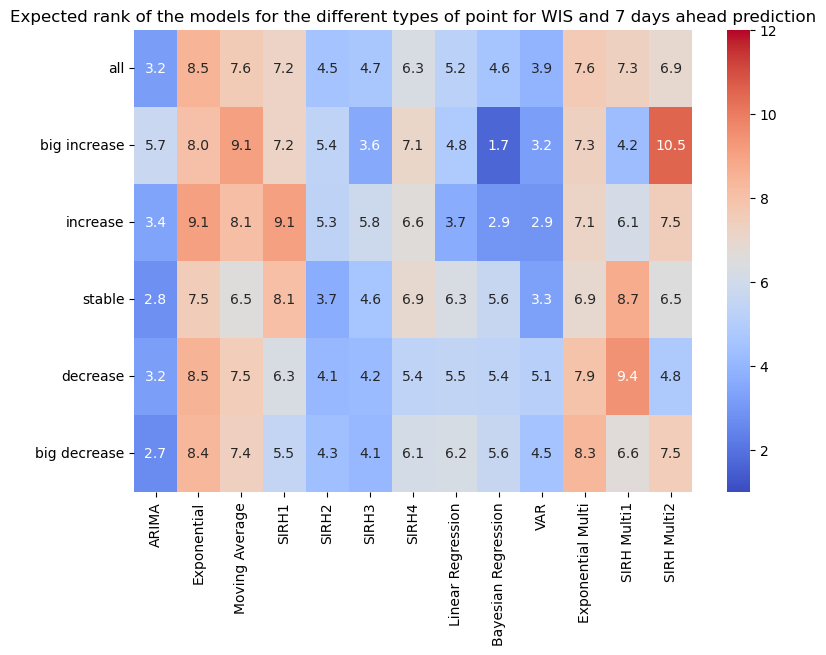
\includegraphics[width=0.7\textwidth]{figures/heatmap_WIS_7.png}
    \caption{Expected rank of the models for each type of point for 7-days ahead predictions and WIS loss}
    \label{fig:heatmap_WIS_7}
\end{figure}


\begin{figure}[h]
    \centering
    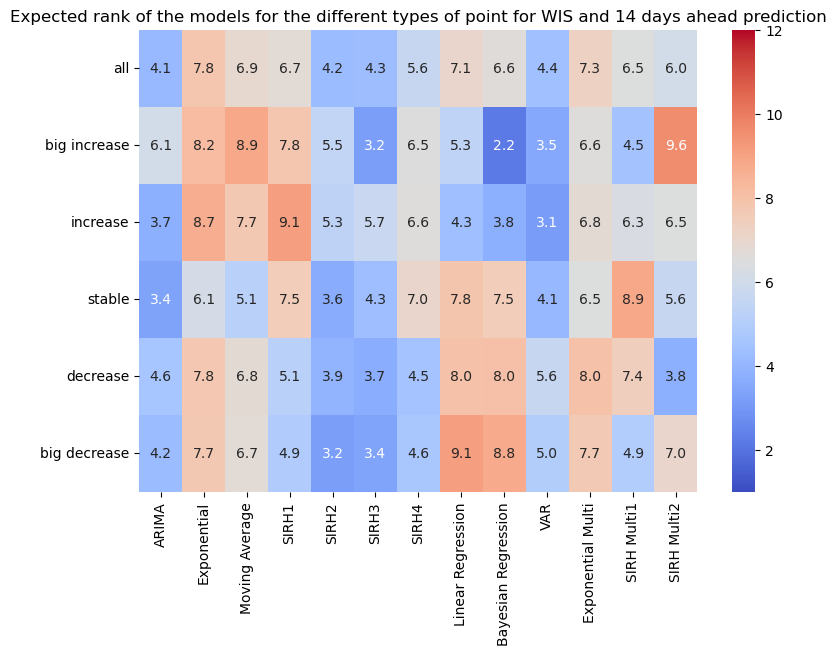
\includegraphics[width=0.7\textwidth]{figures/heatmap_WIS_14.png}
    \caption{Expected rank of the models for each type of point for 14-days ahead predictions and WIS loss}
    \label{fig:heatmap_WIS_14}
\end{figure}



\begin{figure}[h]
    \centering
    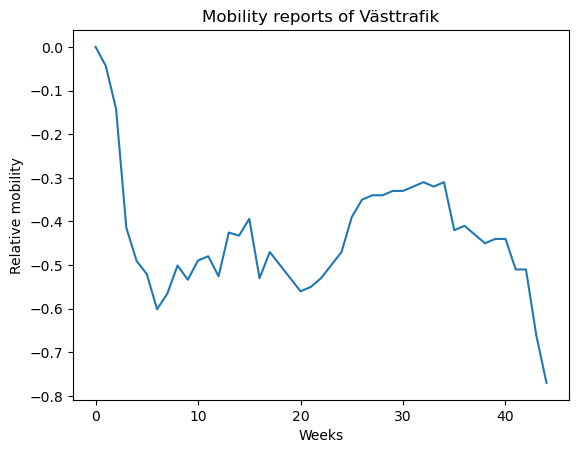
\includegraphics[width=0.5\textwidth]{figures/mobility_reports.png}
    \caption{Mobility reports.}
    \label{fig:mobility_reports}
\end{figure}



\begin{figure}[h!]
    \centering
    % Première sous-figure
    \begin{subfigure}[b]{0.45\textwidth}
      \centering
      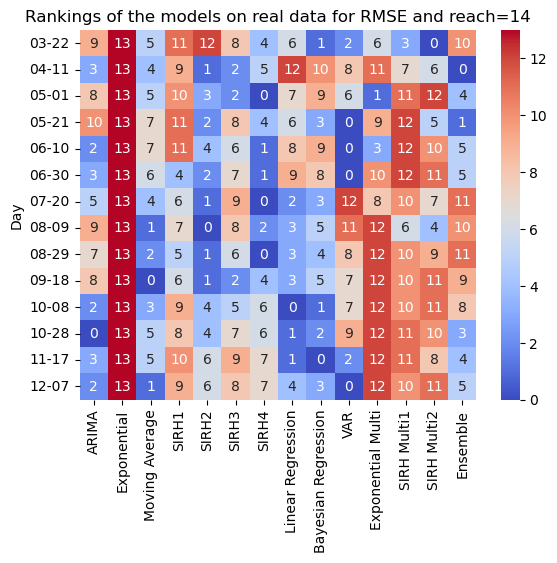
\includegraphics[width=\textwidth]{figures/heatmap_real_14.png}  % Remplacez "image1.png" par le chemin de votre première image
      \caption{Rankings for 7-days ahead predictions}
      \label{fig:sousfig1}
    \end{subfigure}
    \hfill
    % Deuxième sous-figure
    \begin{subfigure}[b]{0.45\textwidth}
      \centering
      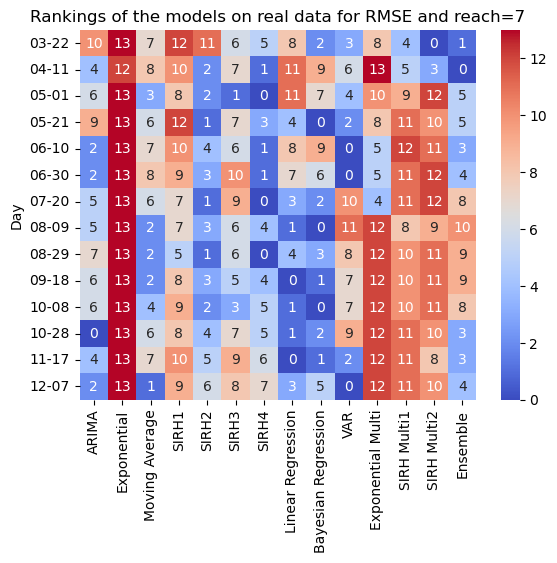
\includegraphics[width=\textwidth]{figures/heatmap_real_7.png}  % Remplacez "image2.png" par le chemin de votre deuxième image
      \caption{Rankings for 14-days ahead predictions}
      \label{fig:sousfig2}
    \end{subfigure}
    \caption{Rankings of the models during the Covid-19 pandemic in Sweden}
    \label{fig:rankings_real_data}
\end{figure}


\begin{figure}[h!]
    \centering
    % Première sous-figure
    \begin{subfigure}[b]{0.5\textwidth}
      \centering
      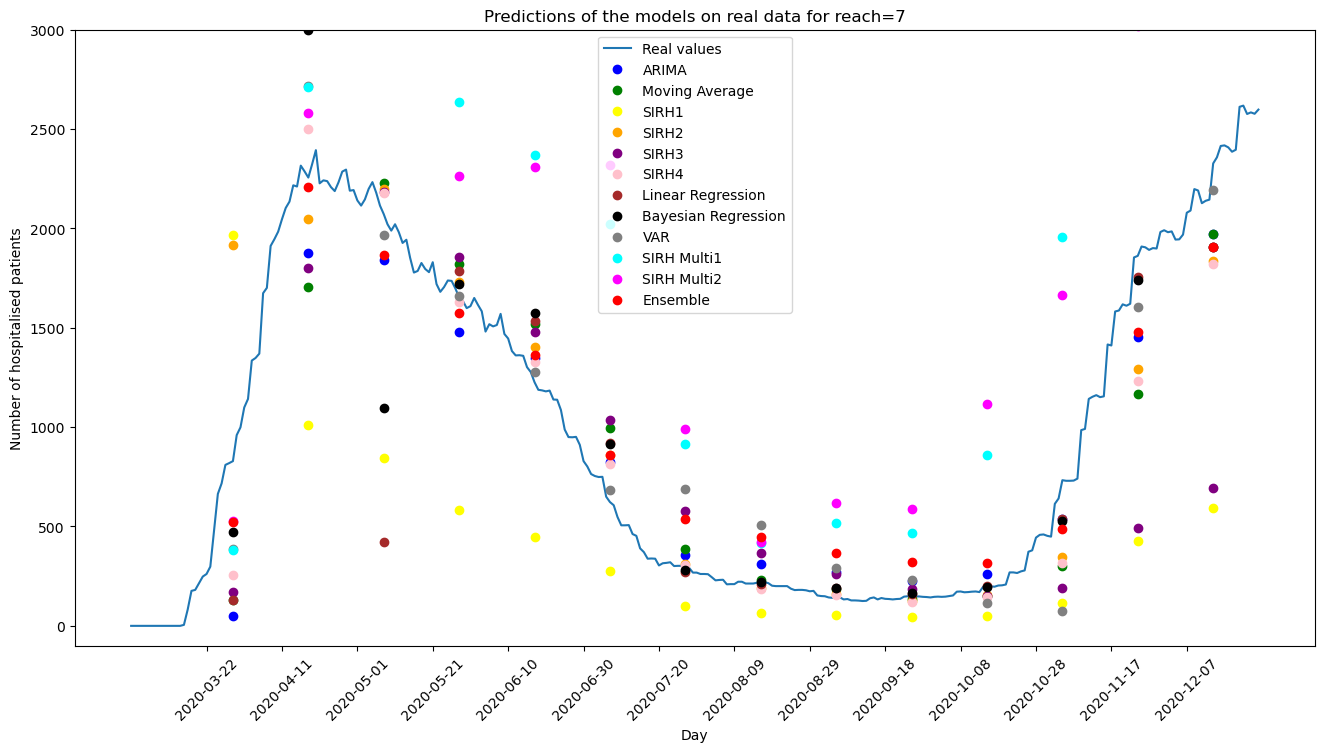
\includegraphics[width=\textwidth]{figures/real_data_7.png}  % Remplacez "image1.png" par le chemin de votre première image
      \caption{Predictions 7-days ahead}
      \label{fig:sousfig1g}
    \end{subfigure}
    \hfill
    % Deuxième sous-figure
    \begin{subfigure}[b]{0.5\textwidth}
      \centering
      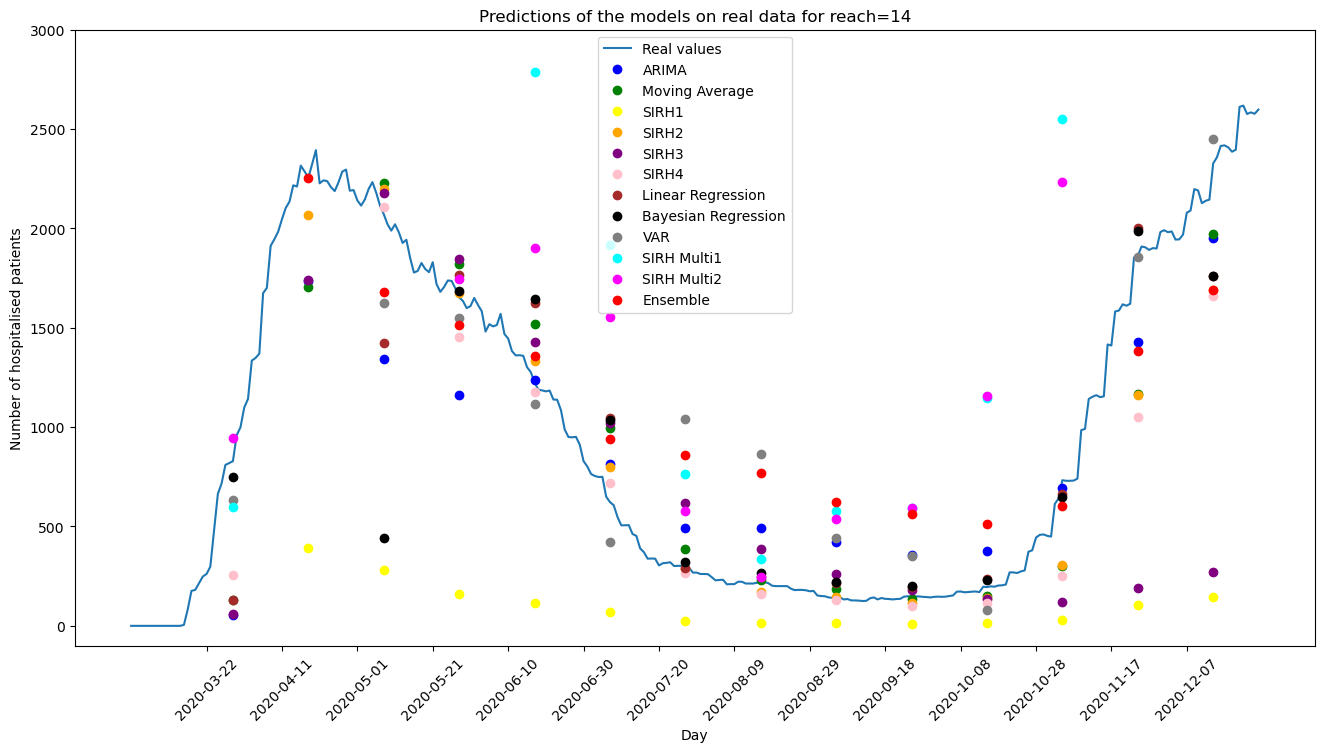
\includegraphics[width=\textwidth]{figures/real_data_14.png}  % Remplacez "image2.png" par le chemin de votre deuxième image
      \caption{Predictions 14-days ahead}
      \label{fig:sousfig2g}
    \end{subfigure}
    \caption{Predictions of the models during the Covid-19 pandemic in Sweden. The y-axis was cut at 3000.}
    \label{fig:real_data}
\end{figure}

